\documentclass{article}

\usepackage{url} 
\usepackage[normalem]{ulem}

\usepackage{pdfpages}
\usepackage{lastpage}
\usepackage{fancyhdr}
\usepackage{ngerman}

\usepackage{xcolor}
\usepackage{listings}
\usepackage{courier}

\usepackage{floatrow}
\usepackage[tableposition=top]{caption}
\floatsetup[table]{capposition=top}

\usepackage{amsmath, amssymb}

\usepackage[utf8]{inputenc}
%\renewcommand{\familydefault}{\sfdefault}

\usepackage[numbib]{tocbibind}


\title{Kalorimetrie}
\author{Johannes Winkler}
\date{}


\newcommand\twodigits[1]{%
   \ifnum#1<10 0#1\else #1\fi
}



\lhead{Kalorimetrie}
\rhead{\today\\Johannes Winkler}
\cfoot{\twodigits{\thepage}~/ \pageref{LastPage}}

\begin{document}

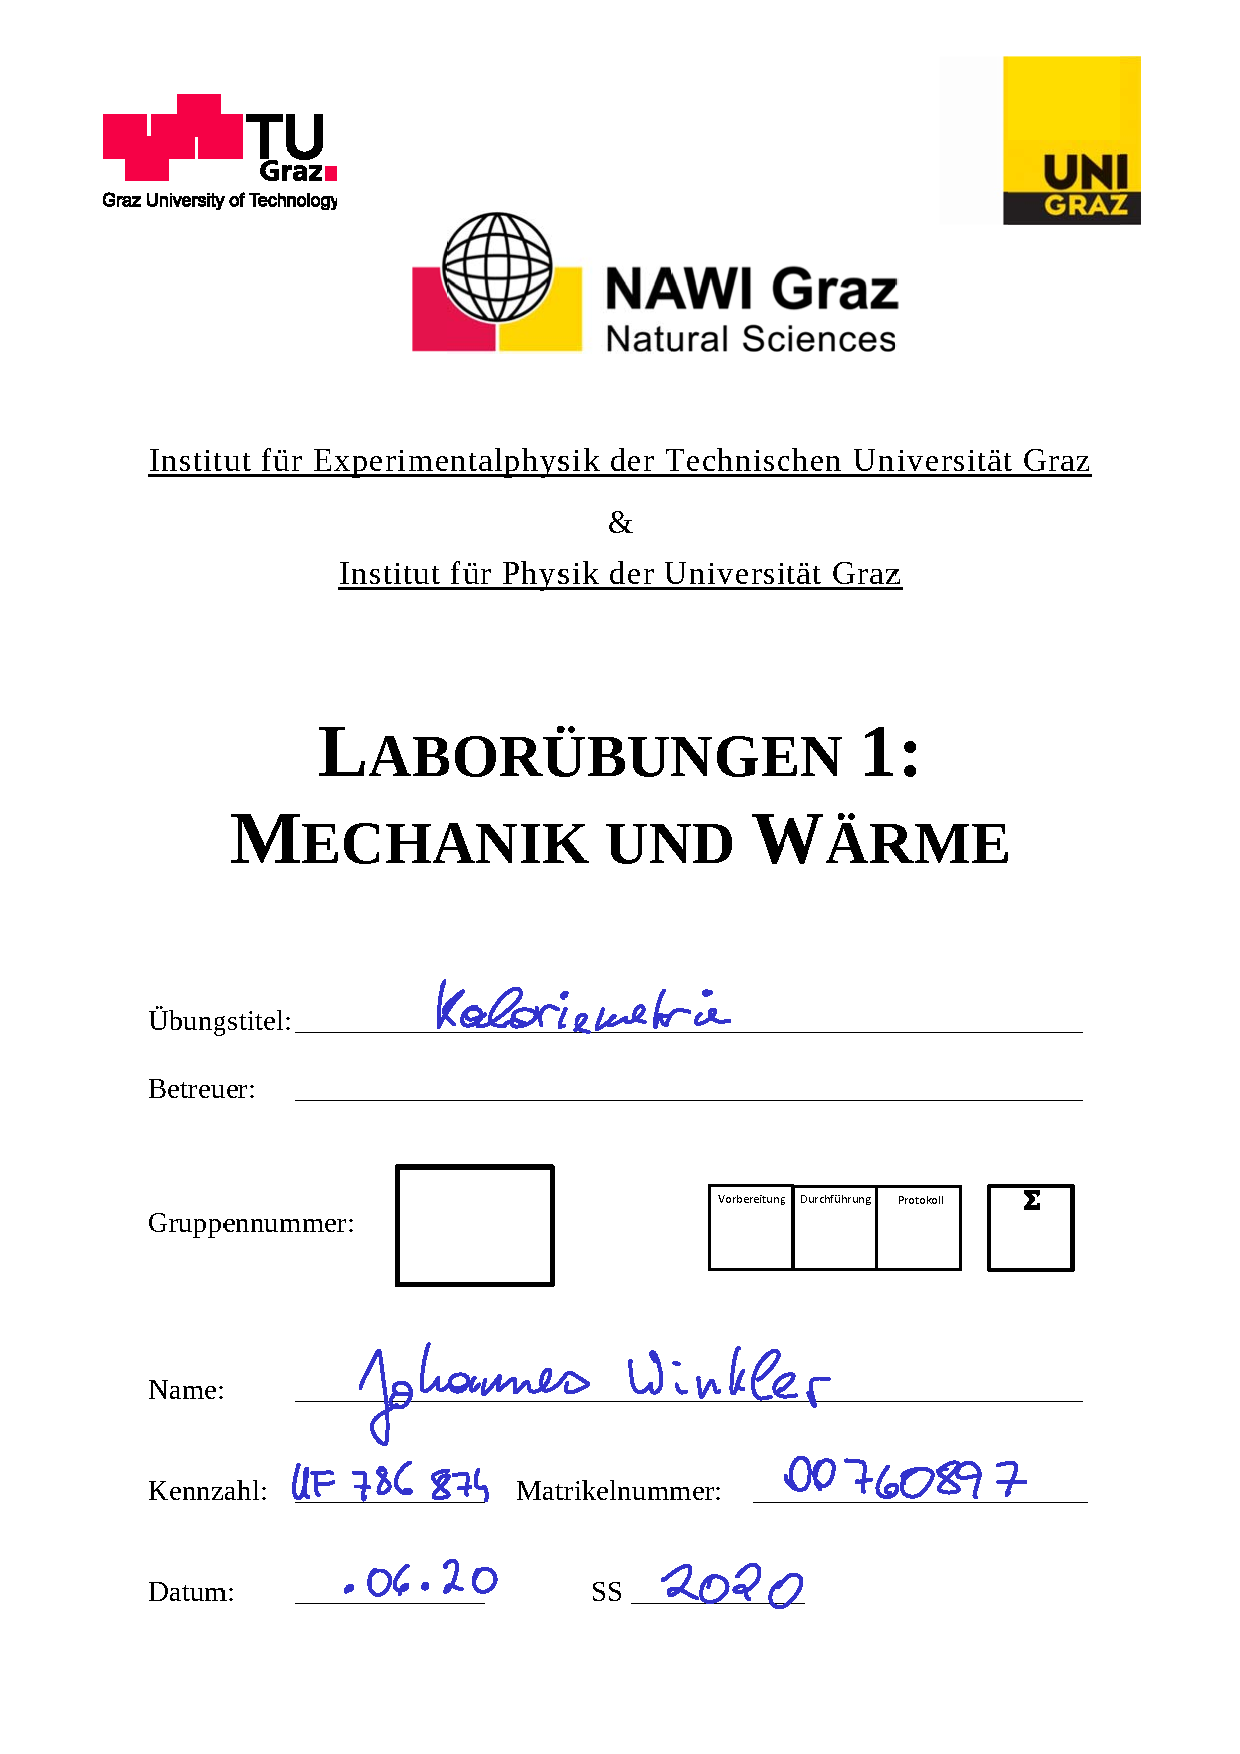
\includepdf[page=-]{deckblatt.pdf} 
 
 
\pagestyle{fancy}


\tableofcontents

\newpage





\section{Aufgabenstellung}

In diesem Versuch ist die Wärmekapazität $C_{th}$ einer Thermoskanne bestimmen. Zusätzlich wird auch die spezifische Wärmekapazität zweier Nahrungsmittel $c_{A1}$ und $c_{A2}$ bestimmt.	


\section{Grundlagen}

Um eine Temperaturerhöhung zu erreichen, muss einem Körper Wärme zugeführt werden. Die Größen Wärme und Temperatur sind proportional, es gilt
\begin{align}
\Delta Q = c\cdot m \cdot \Delta T
\end{align}

Da die Experimente bei Normaldruck erfolgen, sind alle Wärmekapazitäten bei konstantem Atmosphärendruck zu verstehen. Bei Mischungen von Stoffen ist zusätzlich auszugehen, dass Wechselwirkungen vernachlässigt werden, es gilt daher
\begin{align}
Q_{A+B} = Q_A + Q_B
\end{align}
Die Gesamtänderung der Wärme ist dann
\begin{align}
\Delta Q_{A+B} = (c_A \cdot m_A + c_B \cdot m_B)\cdot \Delta T
\end{align}

Daraus lassen sich Wärmekapazitäten bestimmen. Werden zwei Stoffe A und B mit den Temperaturen $T_A$ und $T_B$, so ergibt sich durch die Gesetze der Thermodynamik eine Mischtemperatur $T_M$. Sofern das System abgeschlossen ist (bzw. die Thermoskanne dicht ist), muss die Wärmeenergie erhalten bleiben. 
\begin{align}
E = c_A\cdot m_A \cdot T_A + c_B\cdot m_B \cdot T_B + C_{th} \cdot T_B
\end{align}
wobei der Index $B$ in diesem Fall für Wasser steht. Da das Wasser sich Anfangs in der Thermoskanne befindet, kann man von $T_{th} = T_B$ ausgehen. Nach einiger Zeit gilt
\begin{align}
 E = c_A\cdot m_A \cdot T_M + c_B\cdot m_B \cdot T_M + C_{th} \cdot T_M
\end{align}
Nach der Energieerhaltung gilt
\begin{align}
c_A\cdot m_A \cdot T_A + c_B\cdot m_B \cdot T_B + C_{th} \cdot T_B &=  c_A\cdot m_A \cdot T_M + c_B\cdot m_B \cdot T_M + C_{th} \cdot T_M
\end{align}
Durch Umformen ergibt sich
\begin{align}
\label{eq:ca_formel}
c_A &=  \frac{(c_B\cdot m_B  + C_{th}) \cdot (T_M - T_B)}{m_A \cdot (T_A - T_M)}
\end{align}
Die Wärmekapazität der Thermoskanne kann man durch Umformung nach $C_{th}$ berechnen.
\begin{align}
\label{eq:cth_formel}
C_{th} = \frac{c_A\cdot m_A\cdot (T_A - T_M) + c_B \cdot m_B \cdot (T_B - T_M)}{T_M - T_B}
\end{align}


\section{Beschreibung der Versuchsanordnung}




\begin{figure}[H]
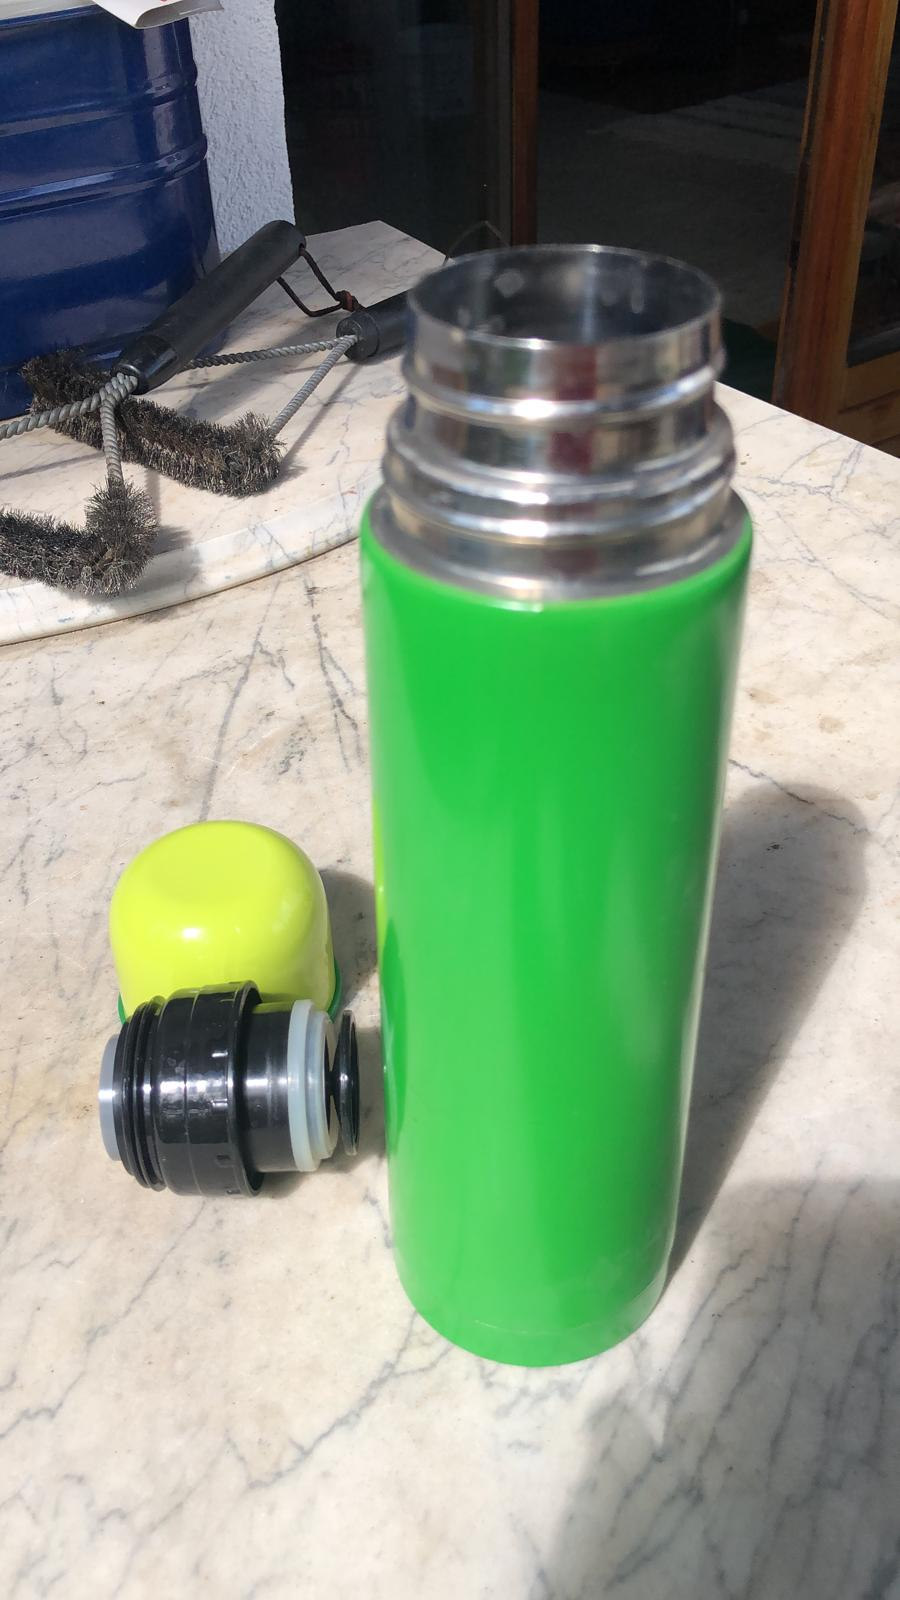
\includegraphics[height=5cm]{thermoskanne.jpg}
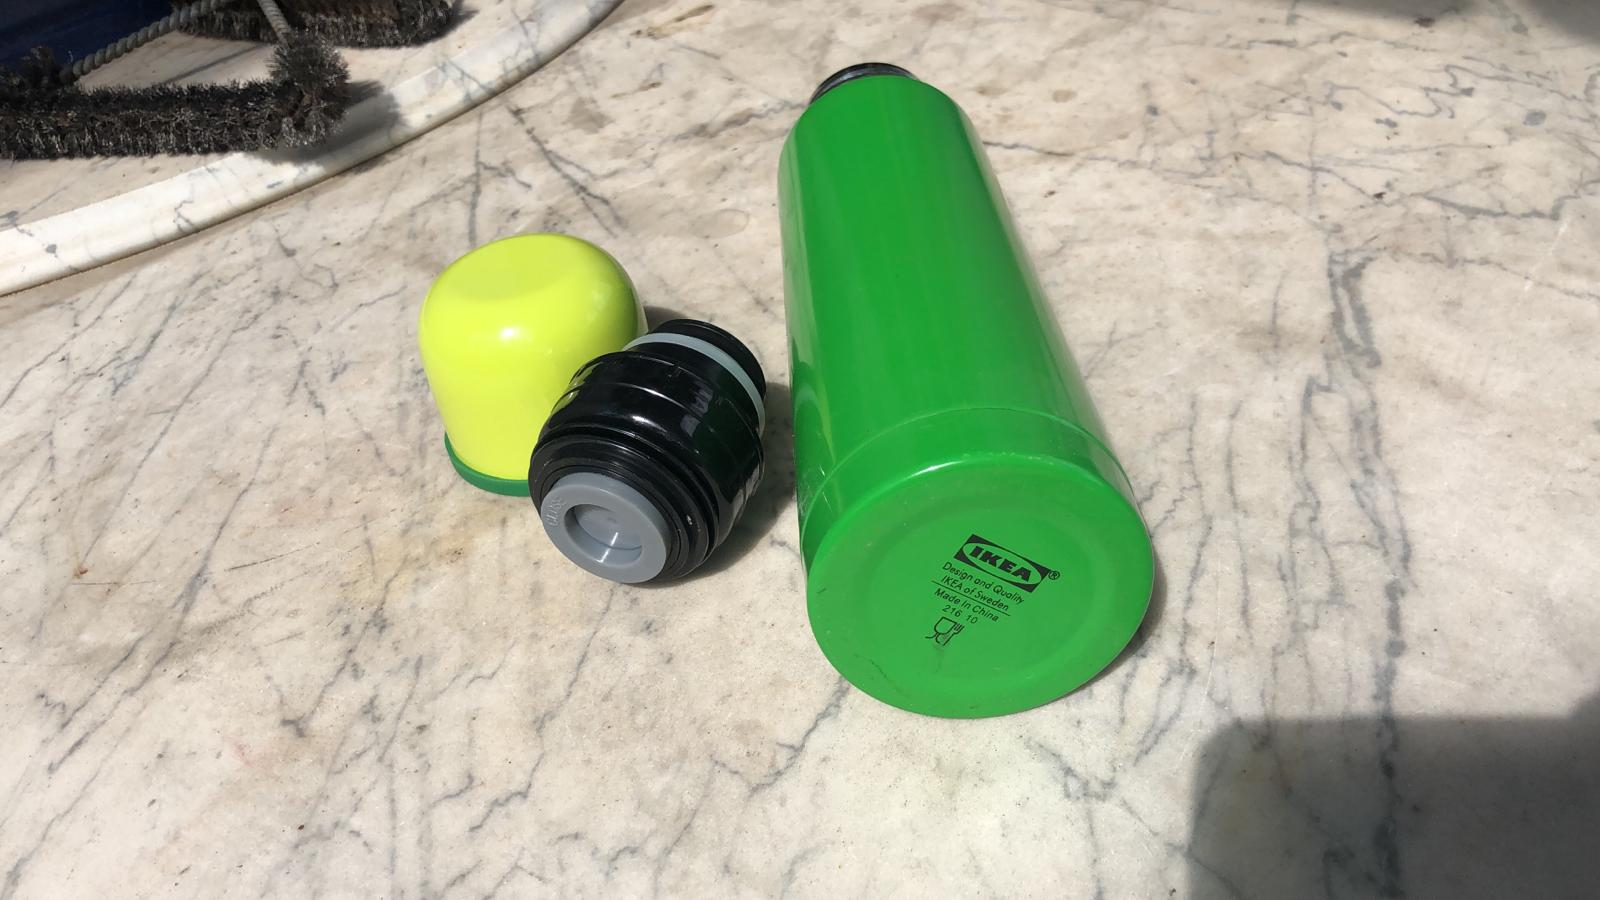
\includegraphics[height=5cm]{thermoskanne2.jpg}
\caption{Thermoskanne (1/2 Liter Füllinhalt)}
\end{figure}

\begin{figure}[H]
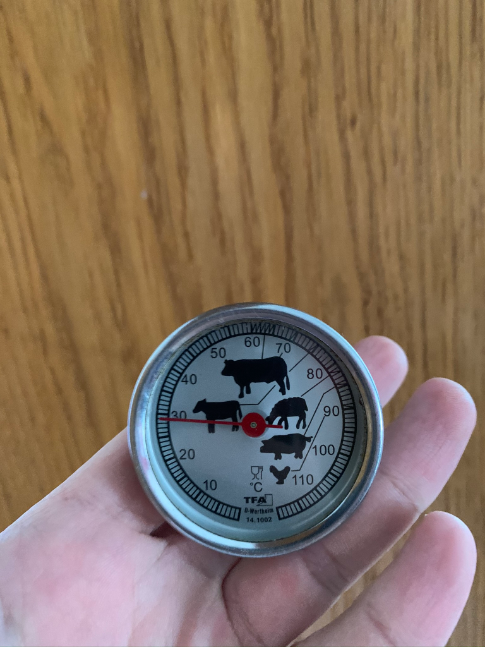
\includegraphics[height=5cm]{thermometer.jpg}
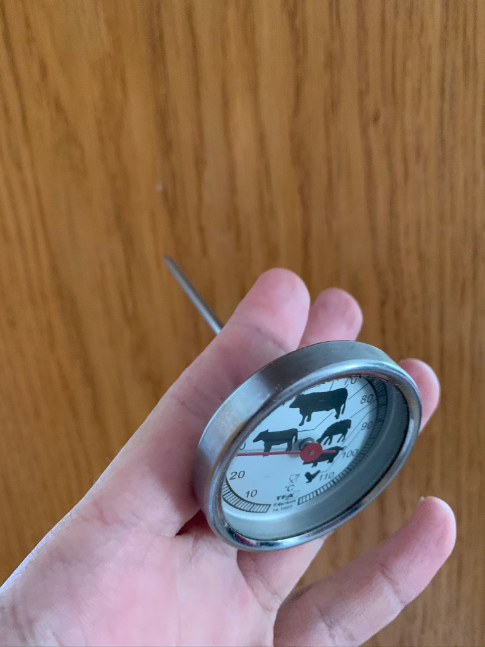
\includegraphics[height=5cm]{thermometer2.jpg}
\caption{Thermometer}
\end{figure}


\begin{figure}[H]
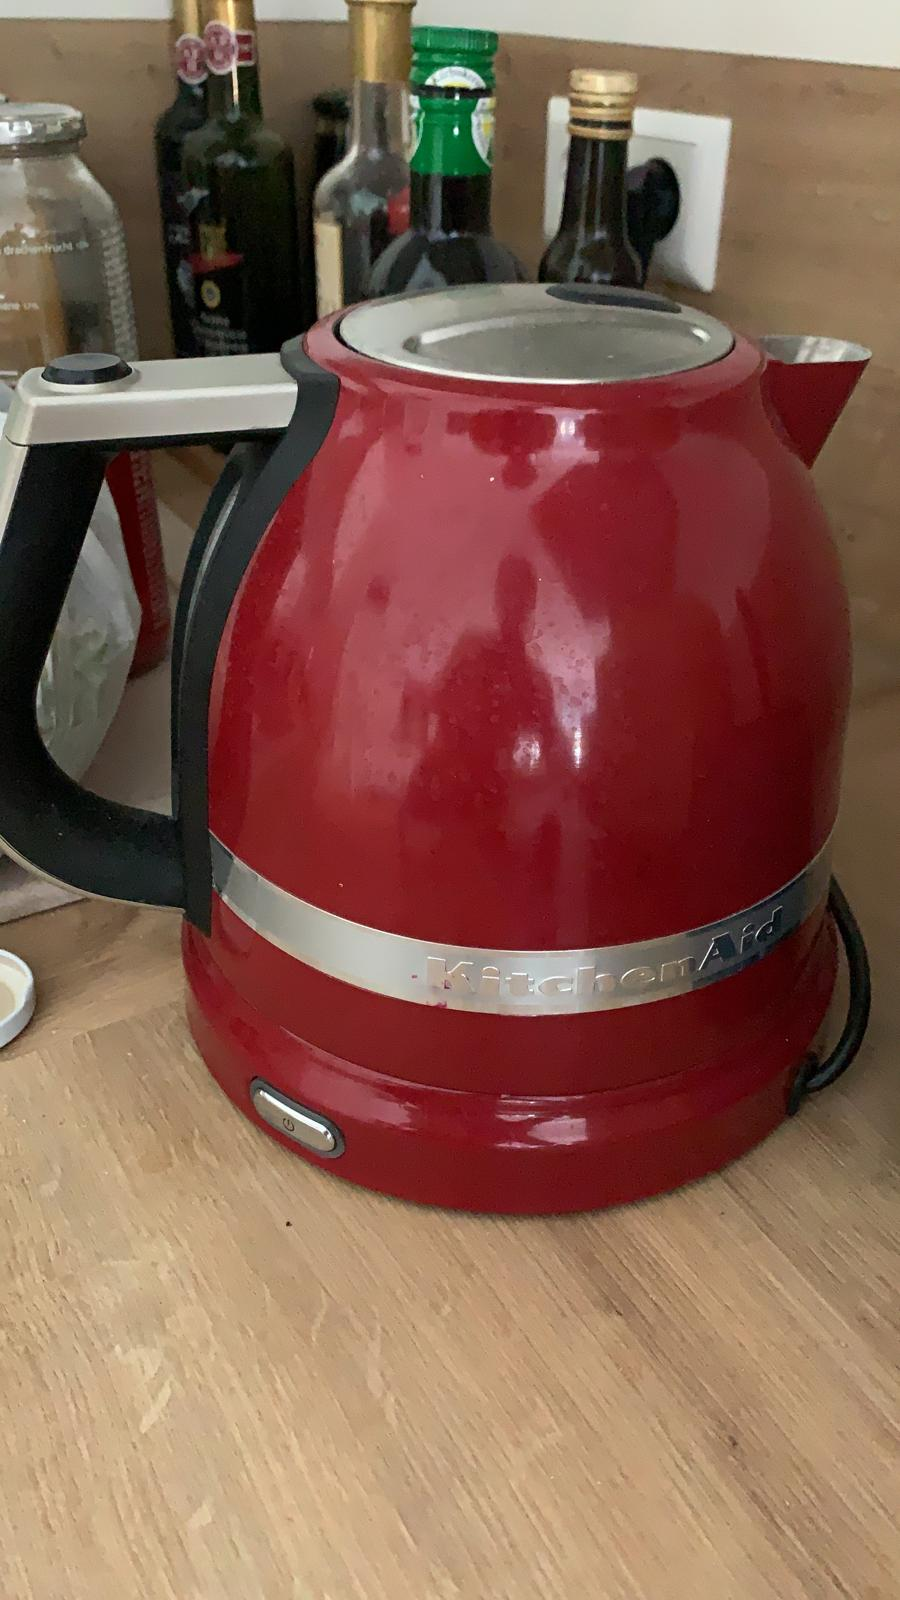
\includegraphics[height=5cm]{wasserkocher1.jpg}
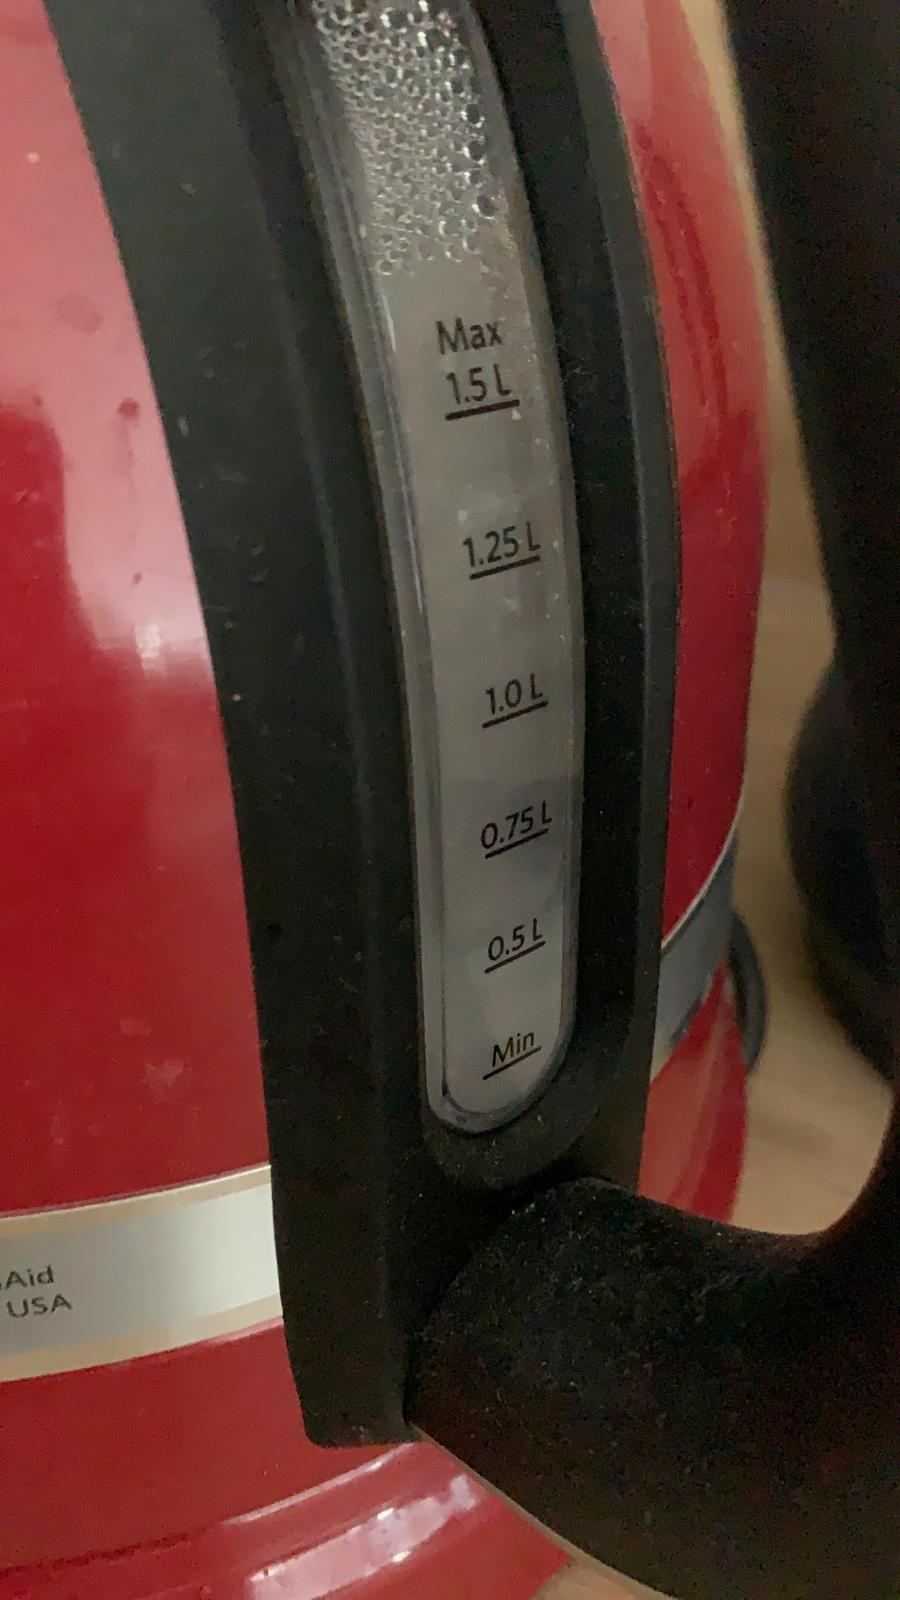
\includegraphics[height=5cm]{wasserkocher2.jpg}
\caption{Wasserkocher (bis zu 1.5~Liter Inhalt)}
\end{figure}


Meine Vorgehensweise zur Berechnung von $C_{th}$:
\begin{itemize}
\item Für Wärmekapazität der Thermoskanne $C_{th}$ wird Formel \eqref{eq:cth_formel} benutzt
\item in diesem Fall sind beide Stoffe Wasser, also $c_A = c_B = 4.2~$kJ/(kg K)
\item ohne es Begründen zu können, vermute ich, dass für optimale Genauigkeit die Anfangstemperaturen $T_A$ und $T_B$ möglichst weit auseinander liegen sollten
\item $T_M$ wird gemessen (Unsicherheit berücksichtigt)
\item Gemäß der Annahme in der Herleitung der Formel muss das Wasser mit dem Index $B$ schon vorher einige Zeit in der Thermoskanne sein, damit diese ebenfalls die Temperatur $T_B$ annimmt. Wasser mit dem Index $A$ wird erst danach dazu gegeben
\item Die genaue Wärmekapazität von Wasser wird in der Literatur recherchiert und später mit Quellenangabe eingefügt.
\end{itemize}

Vorgehensweise für die spezifische Wärmekapazität zweier Lebensmittel $c_{A1}$ und $c_{A2}$
\begin{itemize}
\item Wasser mit Masse $m_B$ in Thermoskanne füllen 
\item warten bis Thermoskanne Temperatur angleicht, Temperatur ist dann $T_B$
\item Es ist $m_B$, $T_B$, $c_B$ bekannt.
\item $m_A$ bekommt man durch Abwiegen des Lebensmittels, $T_A$ mit Hilfe des Bratenthermometers (eventuell lege ich die Lebensmittel vorher in Wasser mit definierter Temperatur ein)
\item $C_{th}$ mit Unsicherheit ist aus Teil 1 bekannt
\item $T_M$ wird gemessen (inkl Unsicherheit)
\item Berechnung von $c_A$ nach Formel \eqref{eq:ca_formel}
\item Unsicherheitsanalyse
\end{itemize}


Im Versuch sollen zwei Gabeln untersucht werden. Die hochwertigere Gabel besteht aus Edelstahl. Jene mit geringerem Wert dürfte aus einer Legierung bestehen, die genaue Zusammensetzung ist aber unbekannt. Es wäre interessant, ob man anhand der gefundenen Wärmekapazität auf das Material 


\begin{figure}[H]
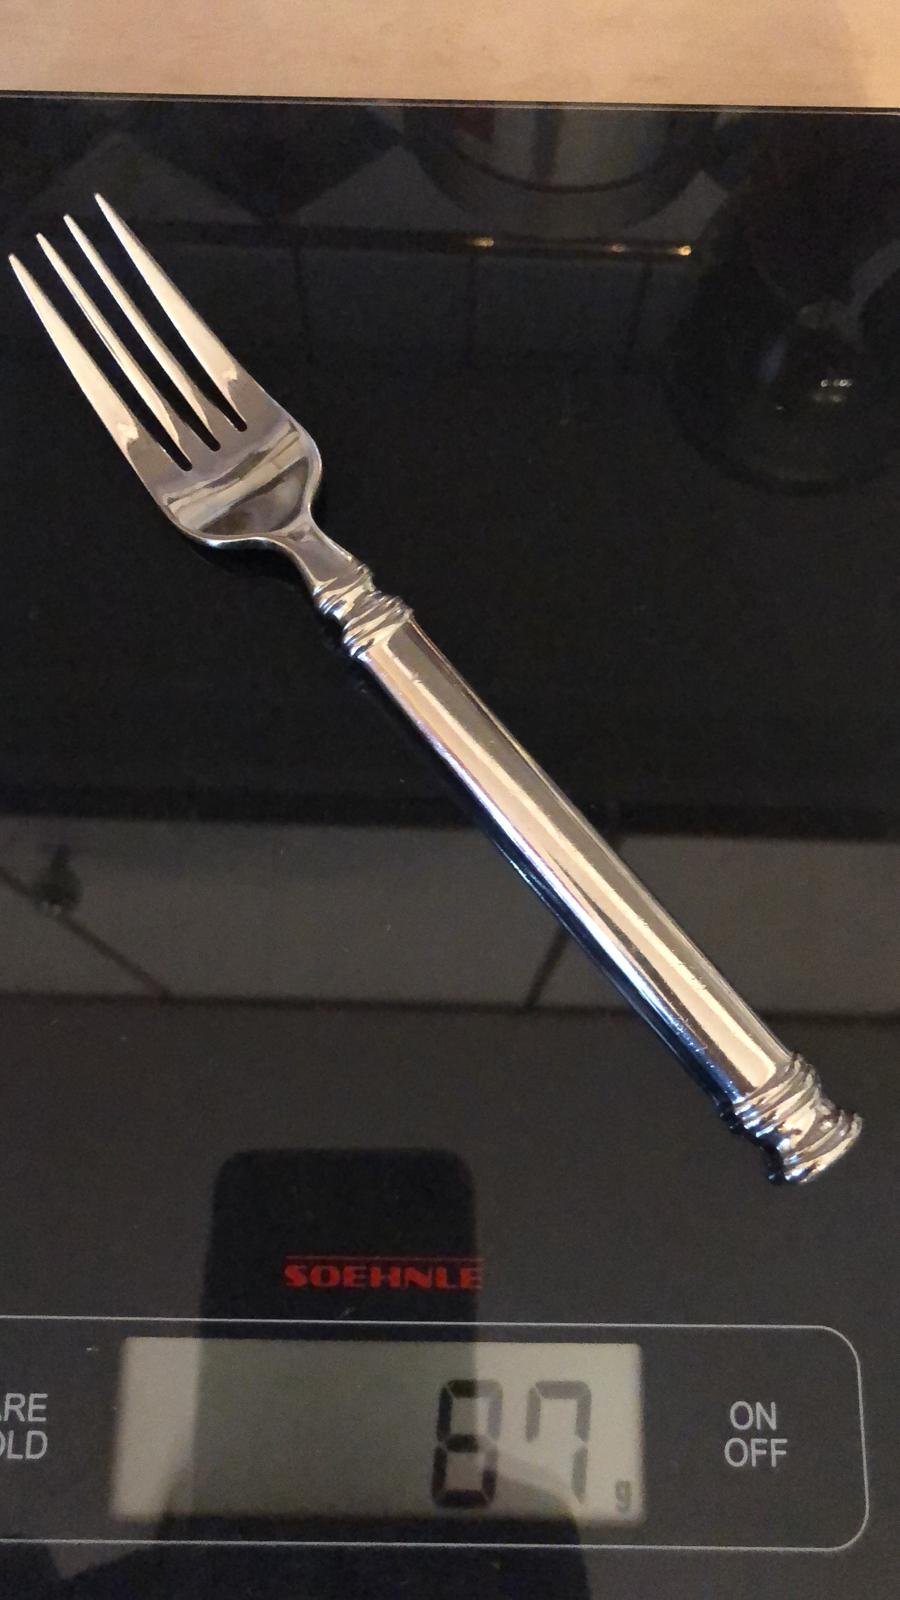
\includegraphics[height=5cm]{gabel1.jpg}
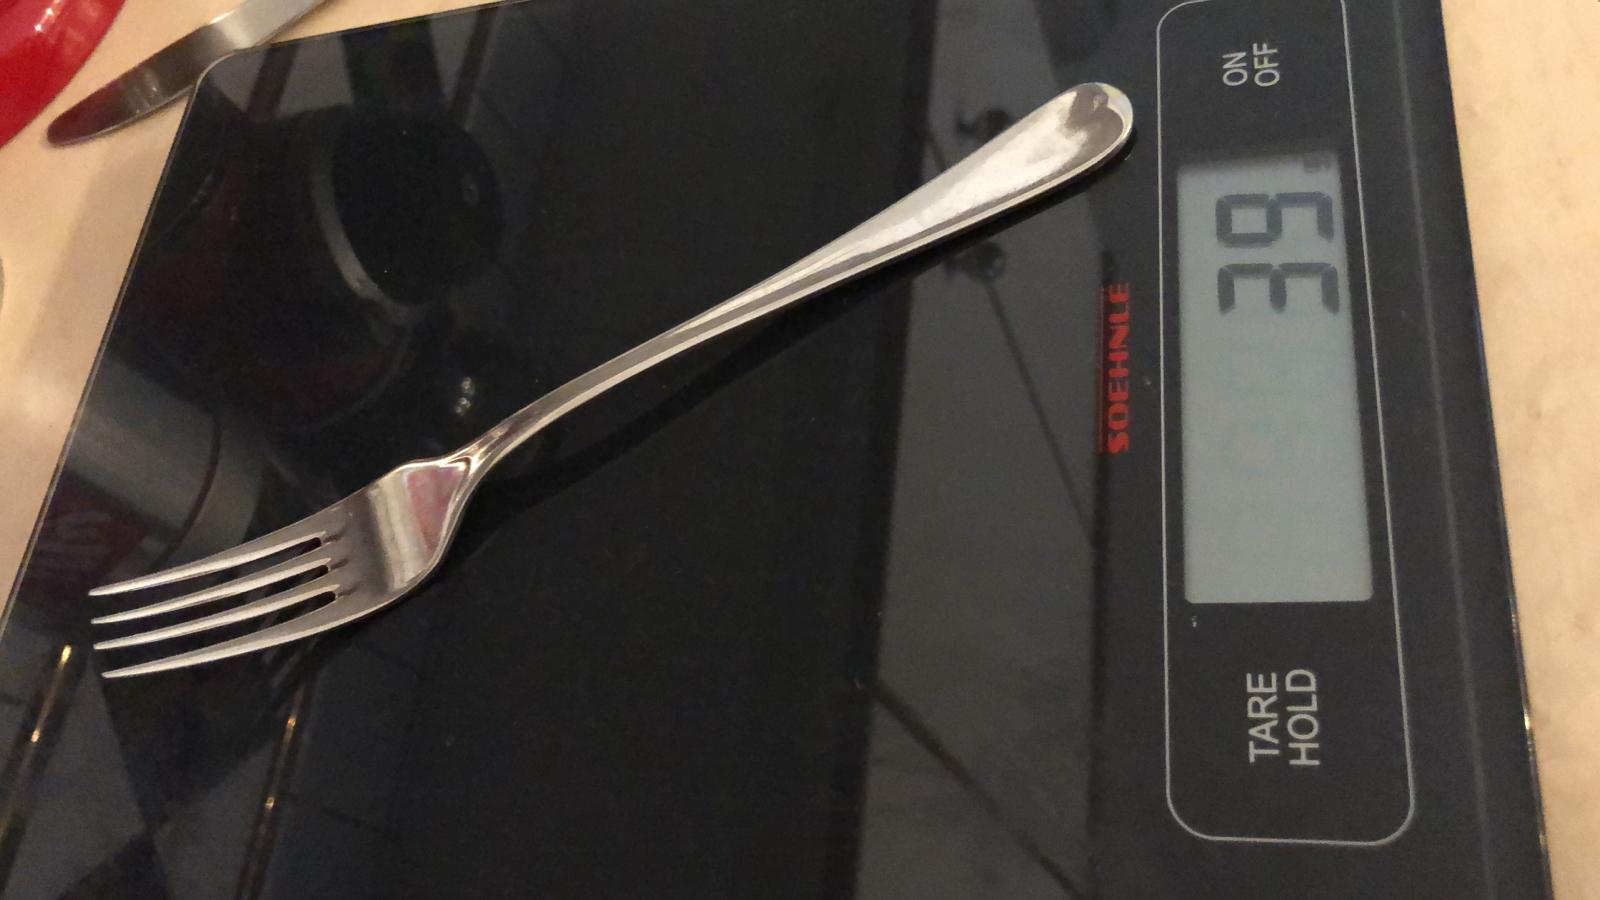
\includegraphics[height=5cm]{gabel2.jpg}
\caption{Die hochwertige Gabel (links) wird im folgenden als Gegenstand A1 bezeichnet. Rechts die weniger hochwertige Gabel, bezeichnet als A2.}
\end{figure}




\begin{figure}[H]
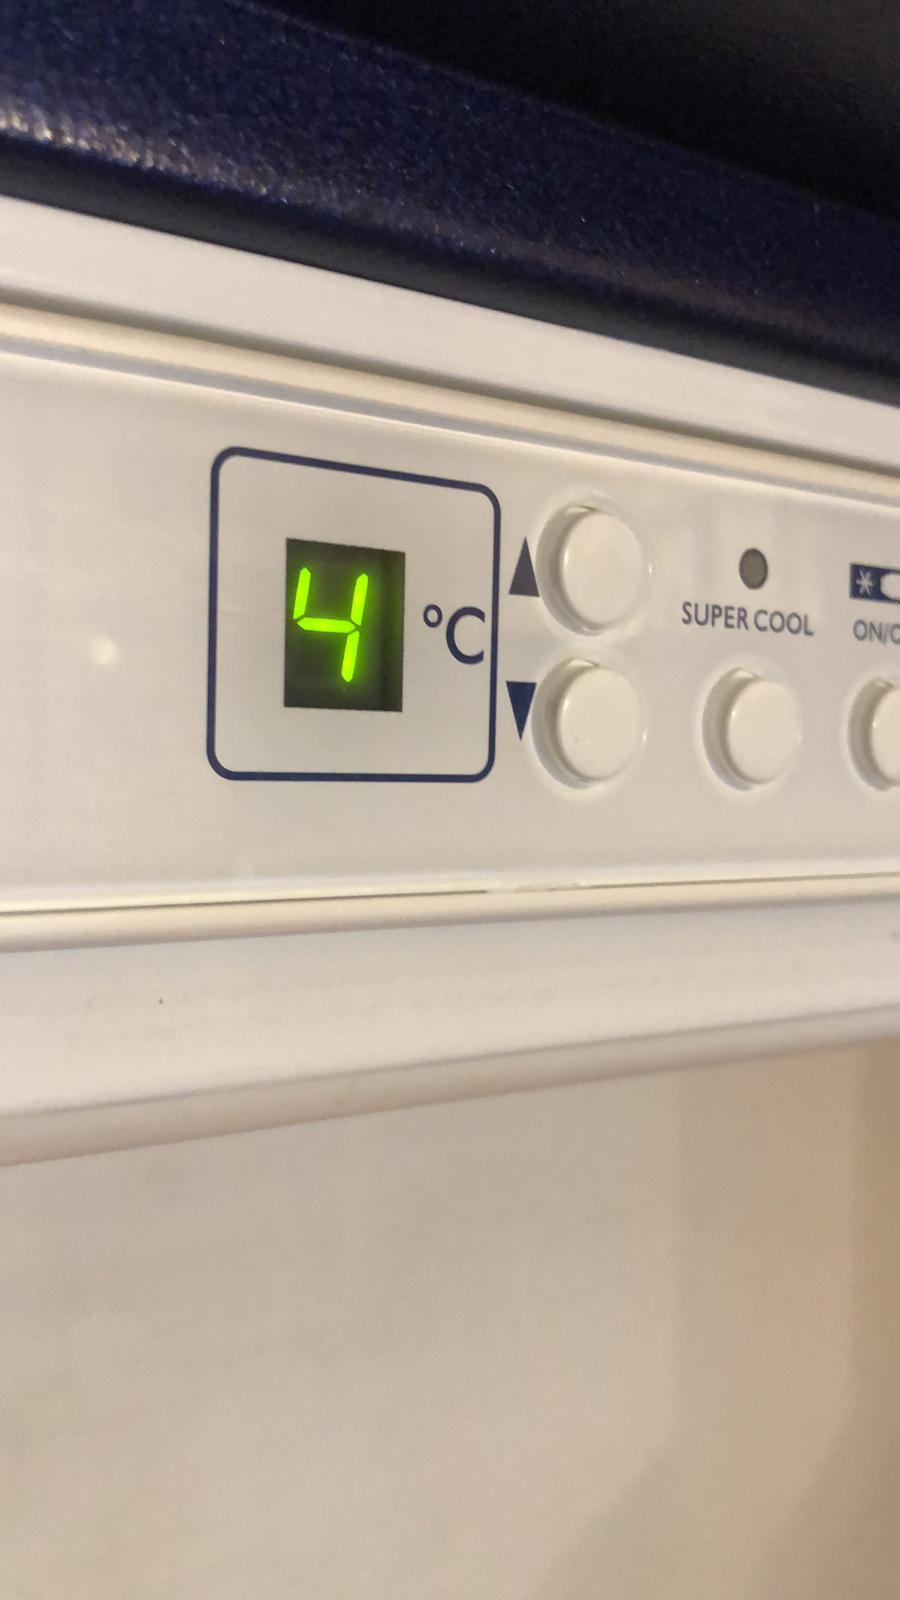
\includegraphics[height=5cm]{kuehlschrank.jpg}
\caption{Kühlschranktemperatur, um eine einheitliche Referenztemperatur zu erzeugen.}
\label{fig:kuehlschrank}
\end{figure}





\section{Geräteliste}




\begin{table}[H]
\caption{Geräteliste}



\begin{tabular}{lll}
Gerät  & Beschreibung \\
\hline
Küchenwaage & von Firma Soehnle, digitales Display, max. Gewicht 5~kg \\
iPhone XS max & Apple, (als Stoppuhr, Wecker)\\
Thermoskanne & 0.5 Liter Inhalt \\
Bratenthermometer & Skala in ${}^\circ$C \\
Wasserkocher & 1.5 Liter Inhalt
\end{tabular}
\end{table}

\newpage
\section{Versuchsdurchführung und Messergebnisse}

Die Wassertemperatur des Wassers $B$ wird zwischen 80 und 90 Grad Celsius gehalten, da mögliche Phasenübergänge Verfälschungen ergeben würden.

\subsection{Wärmekapazität der Thermoskanne}

Zuerst wird $m_B = 500~g$ heißes Wasser $B$ in die Thermoskanne gegeben und diese dicht verschlossen. Für das Abwiegen wurde die Küchenwaage mit Tara-Funktion verwendet. Das Wasser wurde mit dem Wasserkocher erhitzt, jedoch (noch) nicht dessen Temperatur gemessen. Nach $t=5$ Minuten ist davon auszugehen, dass das Wasser $B$ und die Thermoskanne dieselbe Temperatur haben (im Folgenden als $T_B$ bezeichnet). Die im Wasser gemessene Temperatur sind $T_B= 82~^\circ$C.

Nachdem $T_B$ bekannt ist, wird $m_A = 500~g$ Wasser mit der Temperatur $T_A = 54~^\circ$C hinzu gegeben. Nach weiteren 5 Minuten unter Verschluss wird $T_M = 72~^\circ$C gemessen.

\subsection{Wärmekapazität der Gabeln}

Beide Gabeln wurden über Nacht in Wasser eingetaucht im Kühlschrank gelagert. Dieser hat eine Temperatur von $T_{A1} = T_{A2} = 4~^\circ$C (siehe Abbildung~\ref{fig:kuehlschrank}).

Nun wird wieder $m_B = 100~$g heißes Wasser in die Thermoskanne gefüllt und nach 5 Minuten die Temperatur gemessen. Diese ist $T_B=85~^\circ$C. Es wird $m_{A1} = 87~$g von Probe A1 dazugegeben, die sich vorher in Wasser mit der Temperatur $T_{A1} = 4~^\circ$C befunden hat. Daraus ergibt sich die Temperatur $T_{M1} = 83~^\circ$C.

Für die andere Probe wird erneut $m_B = 100~$g heißes Wasser in der Thermoskanne vorbereitet. Nach Temperaturangleichung gilt $T_B = 88~^\circ$C. Probe A2 mit Masse $m_{A2} = 39~$g wird in Wasser mit $T_{A2} = 4~^\circ$C vorbereitet.

\section{Auswertung}

\subsection{Wärmekapazität der Thermoskanne}

Die Wärmekapazität der Thermoskanne kann durch folgende Formel berechnet werden
\begin{align}
C_{th} = \frac{c_A\cdot m_A\cdot (T_A - T_M) + c_B \cdot m_B \cdot (T_B - T_M)}{T_M - T_B}
\end{align}
Nach Einsetzen aller Größen ergibt sich $C_{th} = 1145.45$~J/K. Für die Unsicherheit setzen wir $T_{AM} := T_A - T_M$, $T_{MB} = T_M-T_B$ und berechnen die Unsicherheit von $T_{AM}$ und $T_{BM}$ mit der Annahme, dass die Temperaturdifferenz maximal um ein halbes Kelvin abweicht. Es gilt daher
\begin{align}
C_{th} = \frac{c_A\cdot m_A\cdot T_{AM} - c_B \cdot m_B \cdot T_{MB}}{T_{MB}} = \frac{c_A\cdot m_A\cdot T_{AM}}{T_{MB}} - c_B\cdot m_B
\end{align}
Für die Unsicherheitsanalyse folgt
\begin{align*}
\Delta C_{th} = \frac{\Delta c_A\cdot m_A\cdot T_{AM}}{T_{MB}} + \frac{ c_A\cdot \Delta m_A\cdot T_{AM}}{T_{MB}} + \frac{ c_A\cdot m_A\cdot \Delta T_{AM}}{T_{MB}} + \\ \frac{ c_A\cdot m_A\cdot T_{AM} \cdot \Delta T_{MB}}{T_{MB}^2 } + \Delta c_B\cdot m_B + c_B\cdot \Delta m_B
\end{align*}
mit $\Delta c_A = \Delta c_B = 0.5~\frac{\text{J}}{\text{kg}\cdot\text{K}}$, $\Delta m_A = \Delta m_B = 1~$g, $\Delta T_{AM|MB} = \frac12~$K.
Die Unsicherheit für die Wärmekapazität der Thermoskanne beträgt ca $350~$J/K. Zur besseren Nachvollziehbarkeit ist im Anhang auch ein Python Skript, dass mit den gegebenen Werten die entsprechende Unsicherheit berechnet.

\subsection{Wärmekapazität der Proben}

\begin{align}
c_A &=  \frac{(c_B\cdot m_B  + C_{th}) \cdot (T_M - T_B)}{m_A \cdot (T_A - T_M)}
\end{align}
Auch hier setzen wir $T_{AM} := T_A - T_M$, $T_{MB} = T_M-T_B$ 
Es gilt
\begin{align}
c_A &=  \frac{(c_B\cdot m_B  + C_{th}) \cdot T_{MB}}{m_A \cdot T_{AM}}
\end{align}

Für die Unsicherheit gilt
\begin{align*}
\Delta c_A =
\frac{(c_B\cdot m_B  + C_{th}) \cdot \Delta T_{MB}}{m_A \cdot T_{AM}} +
\frac{\Delta C_{th} \cdot T_{MB}}{m_A \cdot T_{AM}} +
\frac{(\Delta c_B\cdot m_B  ) \cdot T_{MB}}{m_A \cdot T_{AM}} \\
+\frac{(c_B\cdot \Delta m_B ) \cdot T_{MB}}{m_A \cdot T_{AM}}
+\frac{(c_B\cdot m_B  + C_{th}) \cdot T_{MB}\cdot \Delta m_A}{m_A^2 \cdot T_{AM}}
+\frac{(c_B\cdot m_B  + C_{th}) \cdot T_{MB}\cdot \Delta T_{AM}}{m_A \cdot T_{AM}^2}
\end{align*}
Auch hier ist der Rechenweg zur Übersichtlichkeit in Python berechnet.

\newpage
\section{Zusammenfassung und Diskussion}

Für die Wärmekapazität gilt
\begin{align}
C_{th} = (1145.45 \pm 349.76)~\text{J}/\text{K}
\end{align}
Zusätzlich gilt für die Proben
\begin{align}
c_{A1} = (455.54 \pm 225.02)~\text{J/(kg K)} \\
c_{A2} = (483.61 \pm 391.72)~\text{J/(kg K)} 
\end{align}
Da beide Werte ähnlich sind, kann man davon ausgehen, dass die Löffel ungefähr dieselbe Wärmekapazität haben und dass sie dadurch aus einem ähnlichen Material sind, also vermutlich sind beide aus Edelstahl.


~

Es zeigt sich, dass die Unsicherheitsanalyse mit der Größtfehlermethode sehr große Unsicherheiten liefert.

Beim Versuch wurde zusätzlich darauf geachtet, möglichst gleiche Bedingungen zu schaffen. Daher wurden bei beiden Gabeln $m_B = 100~$g verwendet.

~

Wenn man die Thermoskanne näherungsweise als Zylinder mit Innenradius $r=3~$cm und einer Höhe von $h=26~$cm annimmt, dann ergibt sich eine Oberfläche von $\textsc{O} = 447.68~$cm${}^2$. Bei einer Wandstärke von $2~$mm ergibt sich für das Volumen des Materials $V=8.95~$cm${}^3$. Für Eisen mit der Dichte $\rho_\text{Eisen} = 7874~$kg/m${}^3$ erhält man als Masse $m=70.50~$g und der Wärmekapazität $c_\text{Eisen} = 449~\frac{\text{J}}{\text{kg}\cdot\text{K}}$. Daraus ergibt sich eine Wärmekapazität für die Thermoskanne $C = 31.65~$J/K. Der berechnete Wert weicht leider sehr weit davon ab, was mit dem ungenauen Thermometer erklärt werden kann. Für die Dichte und die Wärmekapazität von Eisen wurde Wikipedia (vgl. \cite{wiki_eisen}) konsultiert.



\begin{thebibliography}{9}
\bibitem{demtr1} W. Demtröder, \emph{Experimentalphysik 1: Mechanik und Wärme}, Springer-Spektrum, 8. Auflage, 2018.

\bibitem{giancoli} D. Giancoli, \emph{Physik}, Pearson, 4. Auflage, 2019.

\bibitem{wiki_eisen} \url{https://de.wikipedia.org/wiki/Eisen} (Stand: \today)
\end{thebibliography}



\section*{Anhang: Python Skript}


%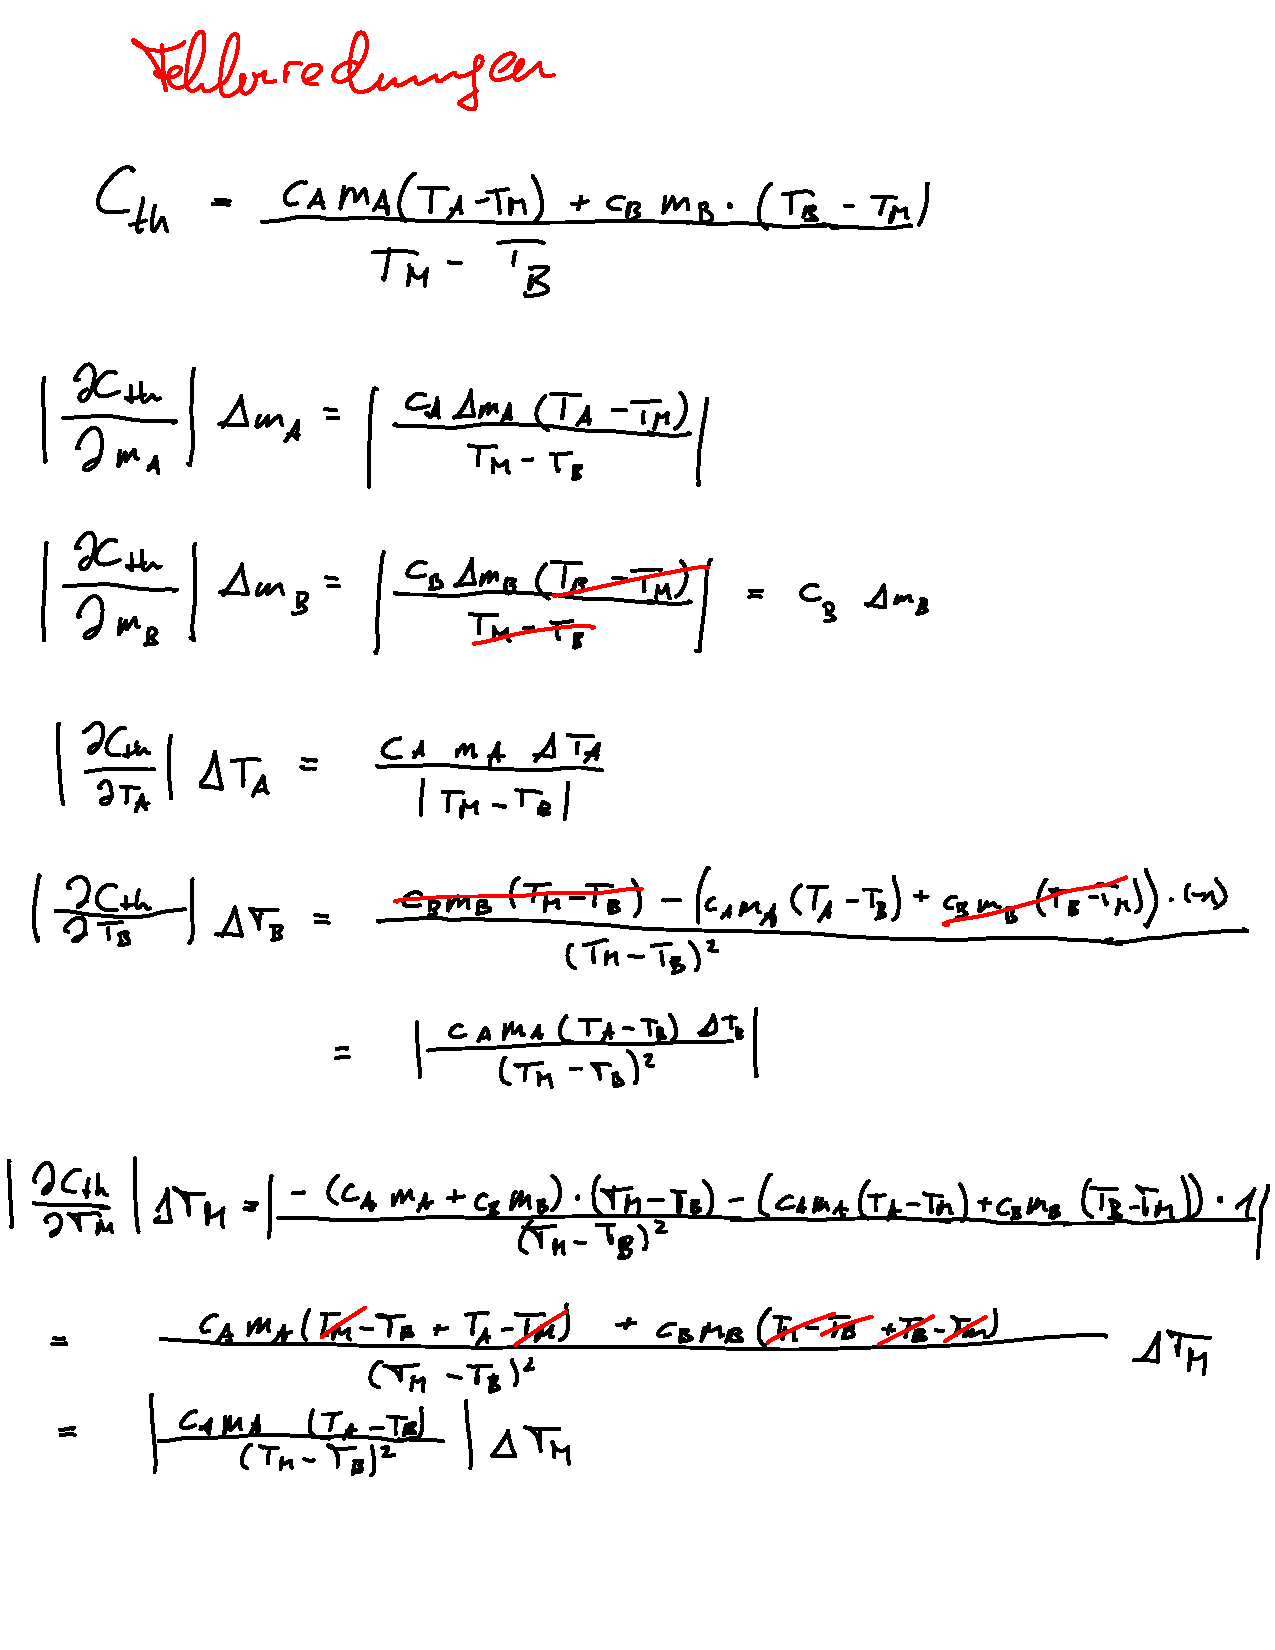
\includepdf[page=-]{nebenrechnungen.pdf} 
\newpage



\definecolor{commentgreen}{RGB}{2,112,10}
\definecolor{eminence}{RGB}{108,48,130}
\definecolor{weborange}{RGB}{255,165,0}
\definecolor{frenchplum}{RGB}{129,20,83}

\lstdefinelanguage{elixir}{
    morekeywords={def, for, range, abs, return},
    otherkeywords={<-,->, |>, \%\{, \}, \{, \, (, )},
    sensitive=true,
    morecomment=[l]{\#},
    morecomment=[n]{/*}{*/},
    morecomment=[s][\color{purple}]{:}{\ },
    morestring=[s][\color{orange}]"",
    commentstyle=\color{commentgreen},
    keywordstyle=\color{eminence},
    stringstyle=\color{red},
	basicstyle=\ttfamily,
	breaklines,
	showstringspaces=false,
	frame=tb
}

\lstinputlisting[language=elixir]{kf_kal.py}

\end{document}
